%%*************************************************************************
%%
%% Analysis of biosignals by means of biologically inspired algorithms
%% V1.0
%% 2011/05/19
%% by Peter Boraros
%% See http://www.pborky.sk/contact for current contact information.
%%
%% Introduction to the methods of analysis of the wide variety signals.
%%
%%
%%*************************************************************************
%% Legal Notice:
%%
%% This code is offered as-is without any warranty either expressed or
%% implied; without even the implied warranty of MERCHANTABILITY or
%% FITNESS FOR A PARTICULAR PURPOSE! 
%% User assumes all risk.
%%
%% This work by Peter Boraros is licensed under a 
%% Creative Commons Attribution-NonCommercial-ShareAlike 3.0 Unported License.
%% http://creativecommons.org/licenses/by-nc-sa/3.0/

\documentclass{beamer}

\usepackage[utf8x]{inputenc}
\usepackage{ifpdf}

\ifpdf
%	\usepackage[pdftex]{graphics}
	\graphicspath{{./img/}}
	\DeclareGraphicsExtensions{.pdf}
\else
%	\usepackage[dvips]{graphics}
	\graphicspath{{./img/}}
	\DeclareGraphicsExtensions{.eps}
\fi
\renewcommand{\figurename}{Fig}

\usetheme{Warsaw}
\title[Analysis of biosignals]{Analysis of biosignals by means of\\ biologically inspired algorithms}
\author{Peter Boraros}
%\institute{}


\begin{document}


\begin{frame}
\titlepage
\end{frame}


\begin{frame}{Outline}
\tableofcontents[pausesections]
\end{frame}

\section{Goals}

\subsection*{Broader definition}
\begin{frame}{Goals}
	\begin{figure}[h]
		\centering
		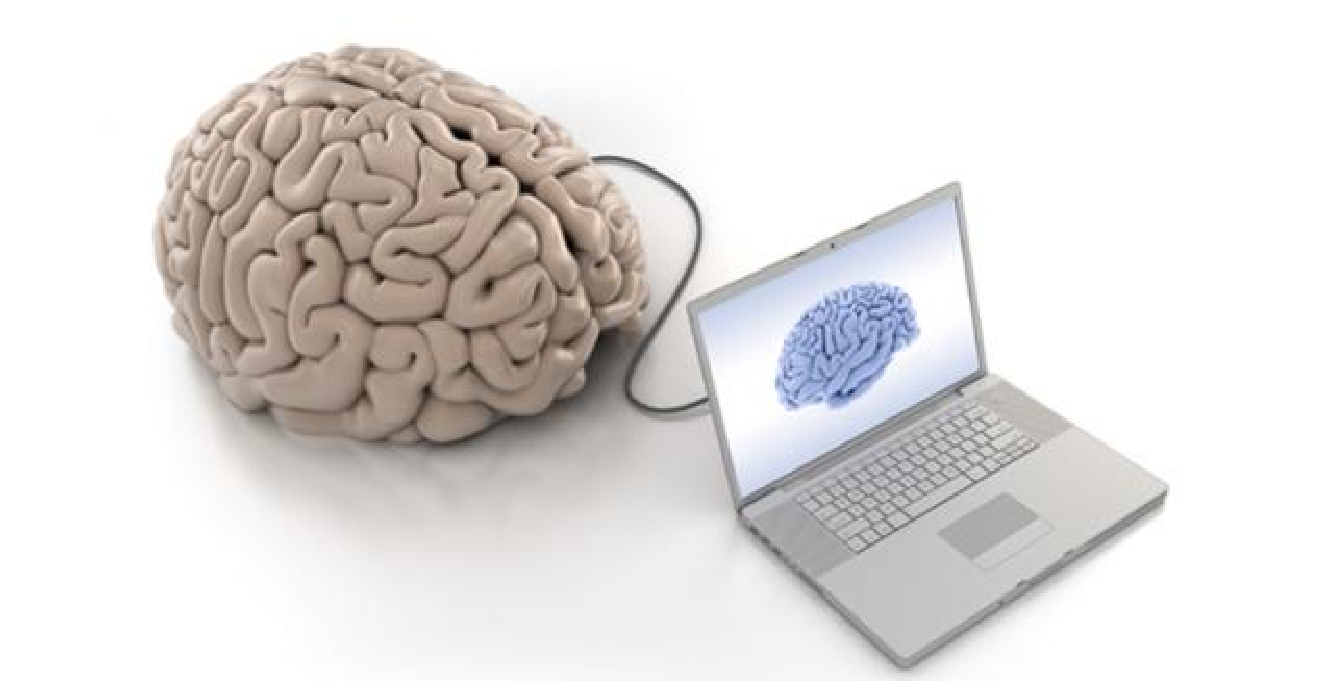
\includegraphics[width=60mm]{brain_computer}
		\label{filters}
	\end{figure}	
	\pause
	\begin{center}
		\textbf{Brain–computer interface}%
		\pause
		\textbf{:}\\
		direct communication pathway between\\ the brain and an device.
	\end{center}
\end{frame}

\subsection*{Narrower definition}
\begin{frame}{Goals (narrower definition) }
\begin{center}
\textbf{Involve} \pause 
an artificial intelligence  in analysis of
\\electroencephalography (EEG) and electromyography (EMG) \pause
\\to control the computer by grimaces or thoughts.\pause
\\\textbf{Eventually} \pause
to support the processing of huge amount of such data 
\\for further research.
\end{center}
\end{frame}

\section{Introduction}

\begin{frame}{Introduction}
\begin{center}
\textbf{EEG} or \textbf{EMG} is electric signal captured in \textbf{time domain} 
ougth to be transformed to \textbf{frequency domain}  and
normalized or equalized to scale.
Used to train \textbf{self-organizing map}
augmented with supervisor 
resulting in classifier that will be able to evaluate EEG or EMG in wider time scale.
\end{center}
\end{frame}

\begin{frame}{Introduction}
\begin{center}
The whole process is controlled by properly configured parameters. The parameters ought to be
found by a \textbf{genetic algorithm}. Additionally \textbf{genetic programming} 
should be involved to modify the process itself.
\end{center}
\end{frame}

\subsection{Fourier transform}
\begin{frame}{Introduction (Fourier transform)}
\alert{not available at this time.. :)}
\end{frame}

\subsection{Self-organizing maps}
\begin{frame}{Introduction (Self-organizing maps)}
\alert{not available at this time.. :)}
\end{frame}

\subsection{Genetic algorithm}
\begin{frame}{Introduction (Genetic algorithm)}
\alert{not available at this time.. :)}
\end{frame}

\subsection{Genetic programming}
\begin{frame}{Introduction (Genetic programming)}
\alert{not available at this time.. :)}
\end{frame}

\section{Implementation}
\subsection{Self-organizing maps}
\begin{frame}{Self-organizing maps}
\alert{not available at this time.. :)}
\end{frame}

\subsection{Genetic algorithm}

\begin{frame}{Genetic algorithm (search space)}
\begin{itemize}
	\item sampling frequency $ f_{samp} $,
	\item time window before fourier transform $ n_w $,
	\item overlap of time windows $ n_o $,
	\item frequency filter after fourier tranform (interval $ \langle f_l, f_h
	\rangle $ defines portion of signal that is kept),
	\item normalisation method (\textit{histogram}, \textit{logaritmic}, 
	\textit{range}, \textit{logistic}),
	\item SOM training algorithm (\textit{batch} or \textit{sequential}),
	\item lattice of SOM (\textit{hexagonal} or \textit{rectangular}),
	\item size of SOM (depends on size of traning dataset).
\end{itemize}
\end{frame}

\begin{frame}{Genetic algorithm (search space)}
	\begin{table}[h]
		\begin{center}
			\begin{tabular}{|l|| l |}
				\hline
				degree of freedom & values \\
				\hline
				\hline
				$ f_{samp} [Hz] $ & 256, 666, 1333, 4000\\
				\hline
				$ n_w $ & 80, 200, 800, 2000 \\
				\hline
				$ n_o $ & 2, 8 \\
				\hline
				$ \langle f_l[Hz], f_h[Hz] \rangle $ & $ \langle 0, 50\rangle $,  
				$ \langle 20, 250\rangle $  \\
				\hline
				normalisation & histogram, logaritmic, range, logistic \\
				\hline
				SOM training algorithm & batch, sequential  \\
				\hline
				SOM lattice & hexagonal, rectangular \\
				\hline
				SOM size  & small, normal \\
				\hline
			\end{tabular}
		\end{center}
	\label{searchspace}
	\end{table}
\end{frame}

\begin{frame}{Genetic algorithm (objectives)}
\begin{itemize}
	\item validation error $ e_v $ of the trained SOM network evaluated by k-fold
	crossvalidation, $ e_v \in \langle 0, 1 \rangle $,
	\item topological error $ e_t \in \langle 0, 1 \rangle $,
	\item mean quantisation error $ e_q $,
	\item window size $ n_w $,
	\item running time $ t_r $ of whole process.
\end{itemize}
\end{frame}

\begin{frame}{Genetic algorithm (fitness function)}
	\[ f = -\ln(e_v+10^{-2 }) - \ln(\Delta t_w+0.5) - (0.7\cdot e_t-0.7) - P(t_r) \]
	\pause
	where:
	\begin{enumerate}
		\item[$ e_v $] validation error
		\item[$ e_t $] topological error
		\item[$ t_r $] running time
		\item[$ \Delta t_w $] window time span\pause
		, expressed as \[  \Delta t_w = \frac{n_w}{f_{samp}}  \]
		\item[$ n_w $] number of captured samples in window
		\item[$ f_{samp} $] sampling frequency
		\item[$ t_r $] running time while $ P(t) $: \[ P(t) = \frac{5}{1+10\cdot e^{6-0.15t}} \]
	\end{enumerate}
\end{frame}

\begin{frame}{Genetic algorithm (fitness function)}
	\[ f = \mathbf{-ln(e_v+10^{-2 })} - \ln(\Delta t_w+0.5) - (0.7\cdot e_t-0.7) - P(t_r) \]
	\centering
	\textbf{Validation error}
	\begin{figure}[h] %
		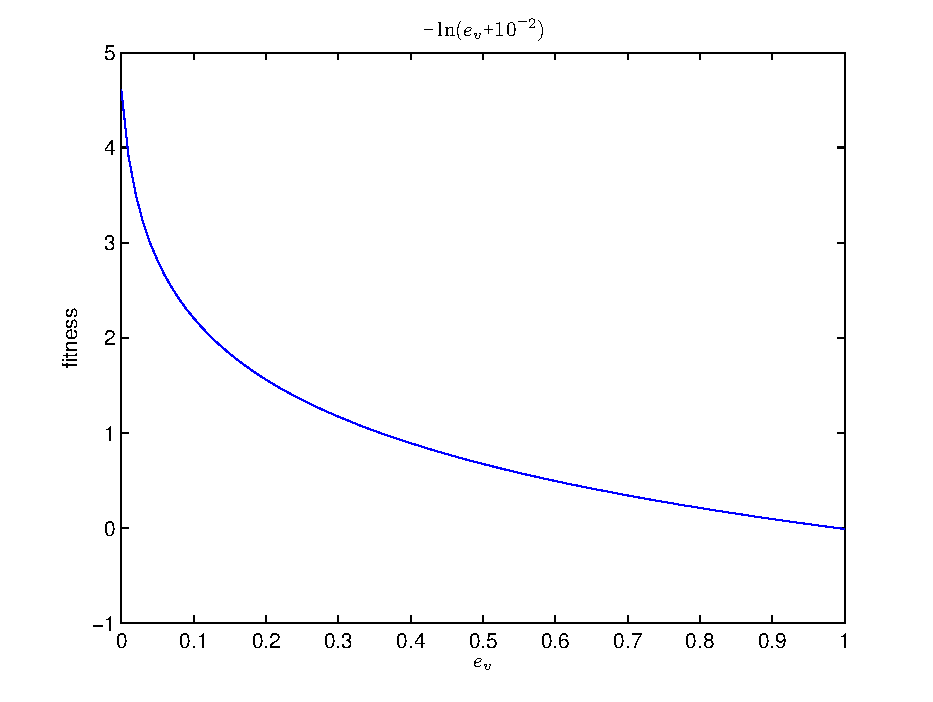
\includegraphics[width=60mm]{fit_ev}
		\label{fit_ev}
	\end{figure}
\end{frame}


\begin{frame}{Genetic algorithm (fitness function)}
	\[ f = -\ln(e_v+10^{-2 }) - \mathbf{ln(\Delta t_w+0.5)} - (0.7\cdot e_t-0.7) - P(t_r) \]
	\centering
	\textbf{Time window width}
	\begin{figure}[h] %
		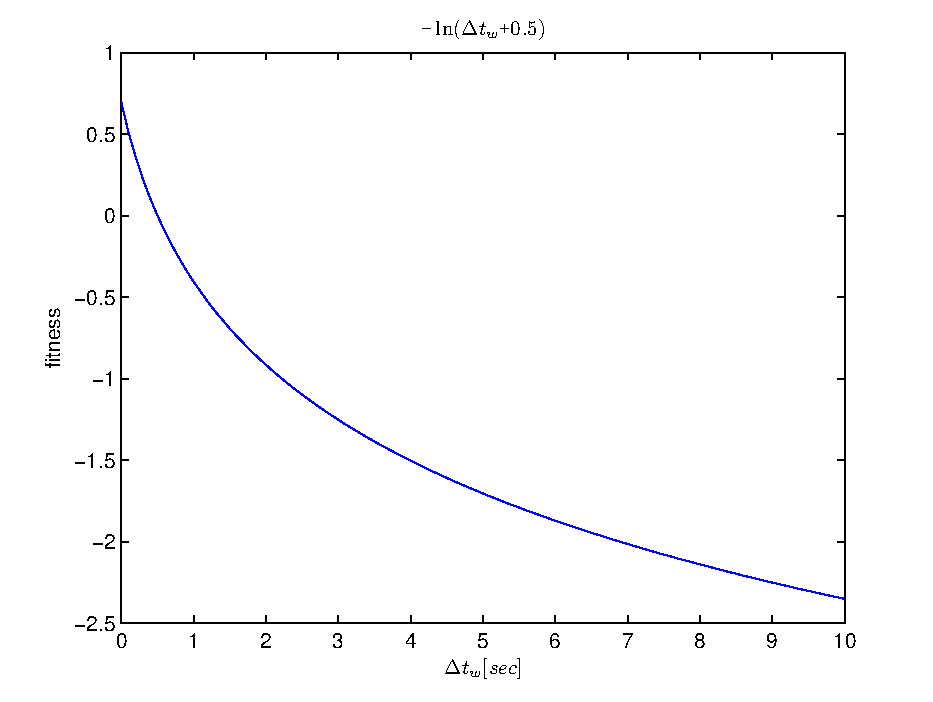
\includegraphics[width=60mm]{fit_tw}
		\label{fit_tw}
	\end{figure}
\end{frame}

\begin{frame}{Genetic algorithm (fitness function)}
	\[ f = -\ln(e_v+10^{-2 }) - \ln(\Delta t_w+0.5) - \mathbf{(0.7\cdot e_t-0.7)} - P(t_r) \]
	\centering
	\textbf{Topological error}
	\begin{figure}[h] %
		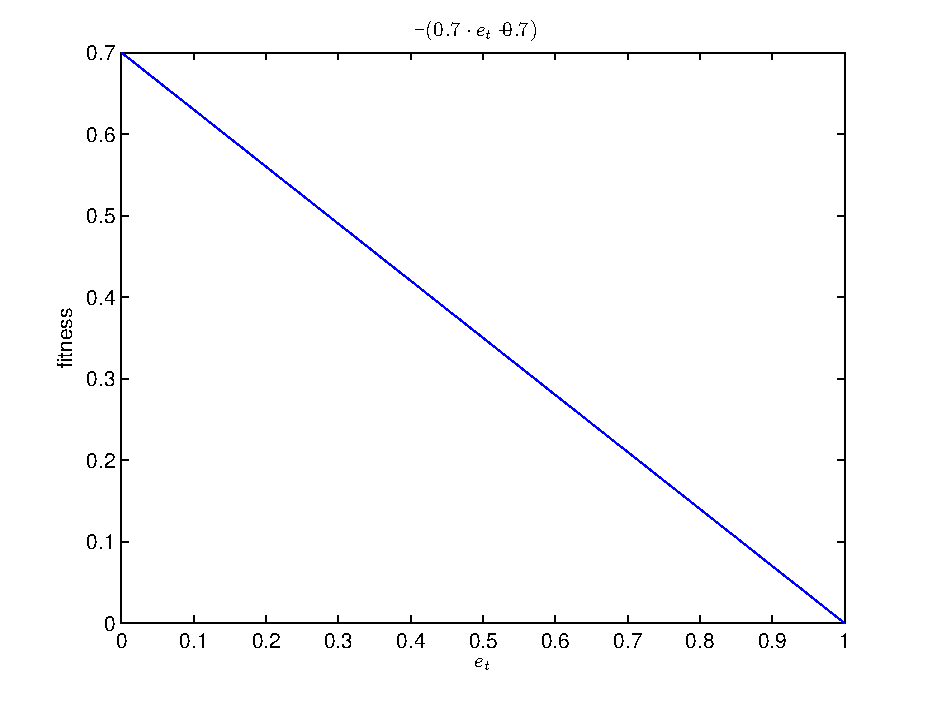
\includegraphics[width=60mm]{fit_et}
		\label{fit_et}
	\end{figure}
\end{frame}

\begin{frame}{Genetic algorithm (fitness function)}
\[ f = -\ln(e_v+10^{-2 }) - \ln(\Delta t_w+0.5) - (0.7\cdot e_t-0.7) - \mathbf{P(t_r)} \]
\centering
\textbf{Running time}
\begin{figure}[h] %
		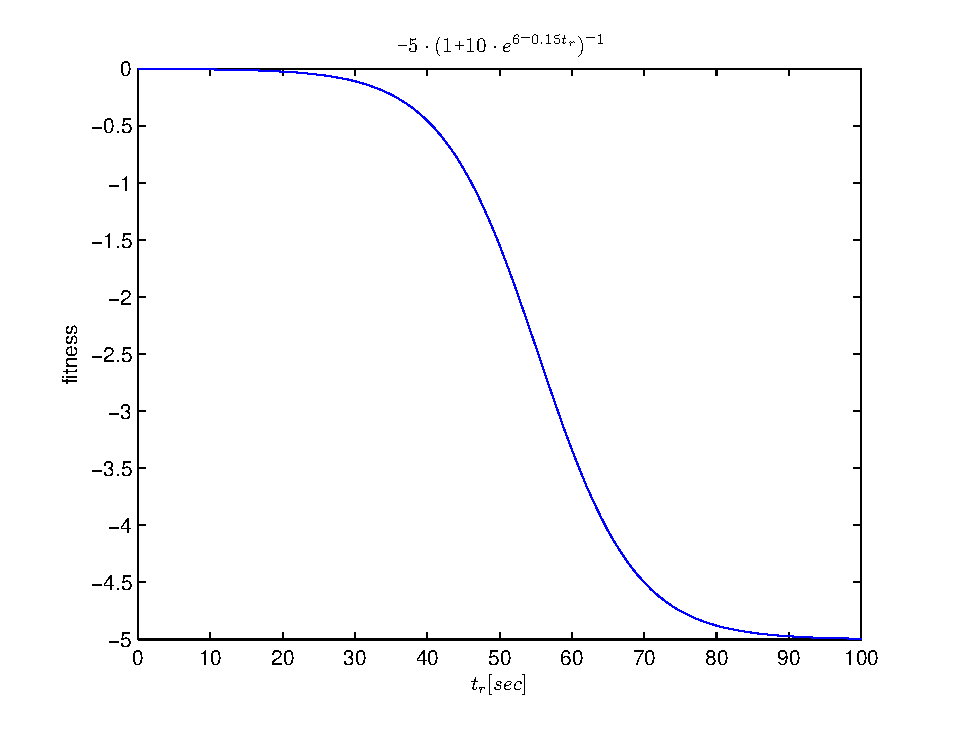
\includegraphics[width=60mm]{fit_tr}
		\label{fit_tr}
\end{figure}
\end{frame}

\begin{frame}{Genetic algorithm (properties)}
\begin{itemize}
	\item genes \pause
	\begin{itemize}
		\item binary strings
		\item integer indices to the search space
	\end{itemize}\pause
	\item given initial population size\pause
	\item random uniform initialization\pause
	\item selection strategy:\pause
	\begin{itemize}
		\item stochastic universal sampling\pause
	\end{itemize}
	\item crossover:\pause
	\begin{itemize}
		\item parents selected using fitness proportionate selection \pause
		 while number of rounds is determined by empiric formula
		\[ N_{pr} = \lceil 0.35\cdot N_{survived} \rceil \]
		where $ N_{survived} $ is the number of survived species\pause
		\item for each parent, its pair is selected by random\pause
		\item randomly selected differing genes are swapped
	\end{itemize}
\end{itemize}
\end{frame}

\begin{frame}{Genetic algorithm (properties)}
\begin{itemize}
	\item crossover:
	\begin{itemize}
		\item parents selected using fitness proportionate selection
		 while number of rounds is determined by empiric formula
		\[ N_{pr} = \lceil 0.35\cdot N_{survived} \rceil \]
		where $ N_{survived} $ is the number of survived species
		\item for each parent, its pair is selected by random
		\item randomly selected differing genes are swapped
	\end{itemize}
	\item mutations:\pause
	\begin{itemize}
		\item species for mutation are selected by:
		\begin{itemize}
			\item using inversed-fitness proportionate selection\pause, where inverse fitness is
			$ f'=-f  $ 
			and count of selection rounds is
			\[ N_{mr} = \lceil n_{mr}\cdot N_{survived} \rceil \] \pause
			where 
			$ n_{mr} $  is the rate of mutation in given population: \pause	
			\[ n_{mr} = 0.05+\dfrac{0.25}{10\cdot e^{0.11\cdot i_{gen}-7}}\]
			and
			$ i_{gen} $ is the actual generation.
		\end{itemize}
	\end{itemize}
\end{itemize}
\end{frame}

\begin{frame}{Genetic algorithm (properties)}
	\centering
	\textbf{Rate of mutations}\\
	\[ n_{mr} = 0.05+\dfrac{0.25}{10\cdot e^{0.11\cdot i_{gen}-7}}\]
	\begin{figure}[h] %
		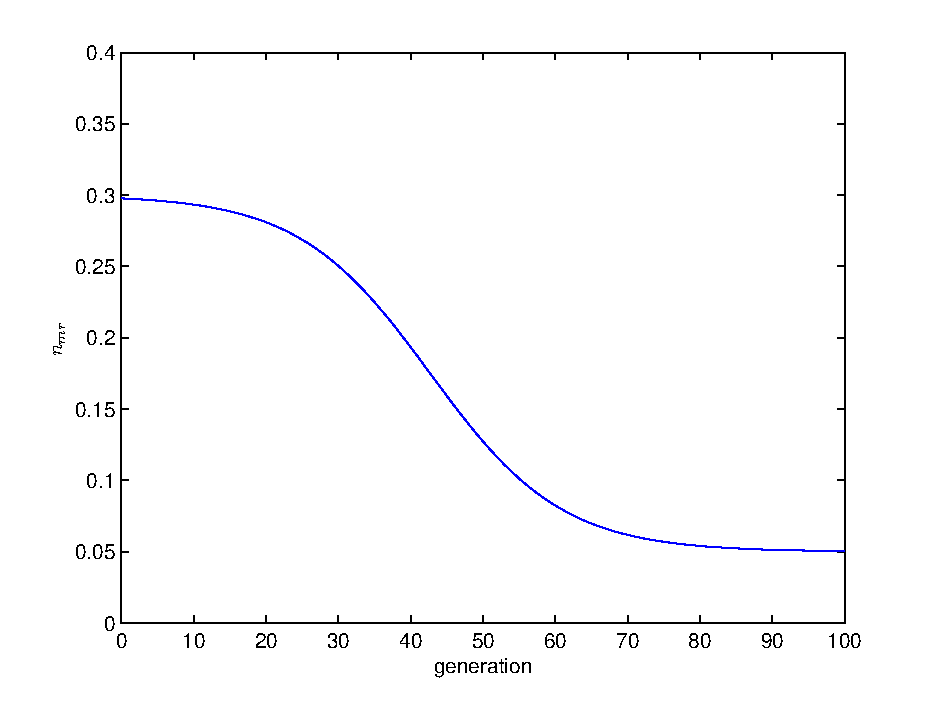
\includegraphics[width=60mm]{mut_r}
		\label{mut_r}
	\end{figure}
\end{frame}

\begin{frame}{Genetic algorithm (properties)}
\begin{itemize}
	\item mutations:
	\begin{itemize}
		\item species for mutation are selected by:
		\begin{itemize}
			\item using inversed-fitness proportionate
			selection, where inverse fitness is
			$ f'=-f  $
			and count of selection rounds is
			\[ N_{mr} = \lceil n_{mr}\cdot N_{survived} \rceil \]
			where 
			$ n_{mr} $  is the rate of mutation in given population denoted as:			
			\[ n_{mr} = 0.05+\dfrac{0.25}{10\cdot e^{0.11\cdot i_{gen}-7}}\]
			where
			$ i_{gen} $ is the actual generation.\pause
			\item from the actual offsprings with probability of mutation for each one:
			$ P_{mo} = n_{mr} $.
		\end{itemize}\pause
		\item each bit is flipped with fixed probability $ P_{mb} = 0.2 $.\pause
	\end{itemize}
	\item stop condition:\pause
	\begin{itemize}
		\item fitness of \textbf{best-fit species} for given interval of generations has \textbf{not} changed.
	\end{itemize}	
\end{itemize}
\end{frame}

\begin{frame}{Genetic algorithm (experiments)}
	\centering
	\textbf{Convergence curve} - single run, agregations in generations\\
	\begin{figure}[h] %
		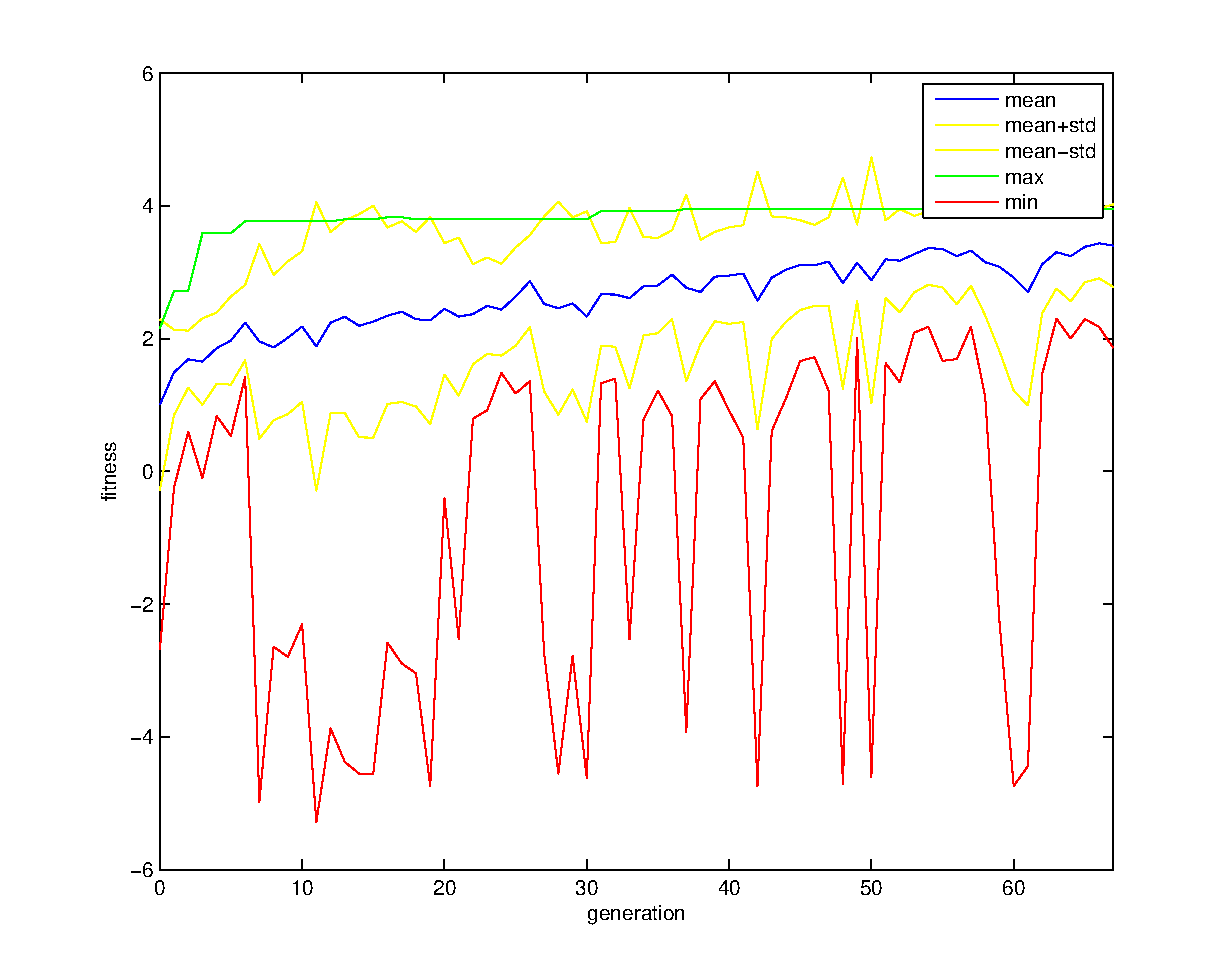
\includegraphics[width=80mm]{ga_conv_curve_s}
		\label{ga_conv_curve_r}
	\end{figure}
\end{frame}

\begin{frame}{Genetic algorithm (experiments)}
	\centering
	\textbf{Convergence curve} - 100 runs, agregations over best-fit species
	\begin{figure}[h] %
		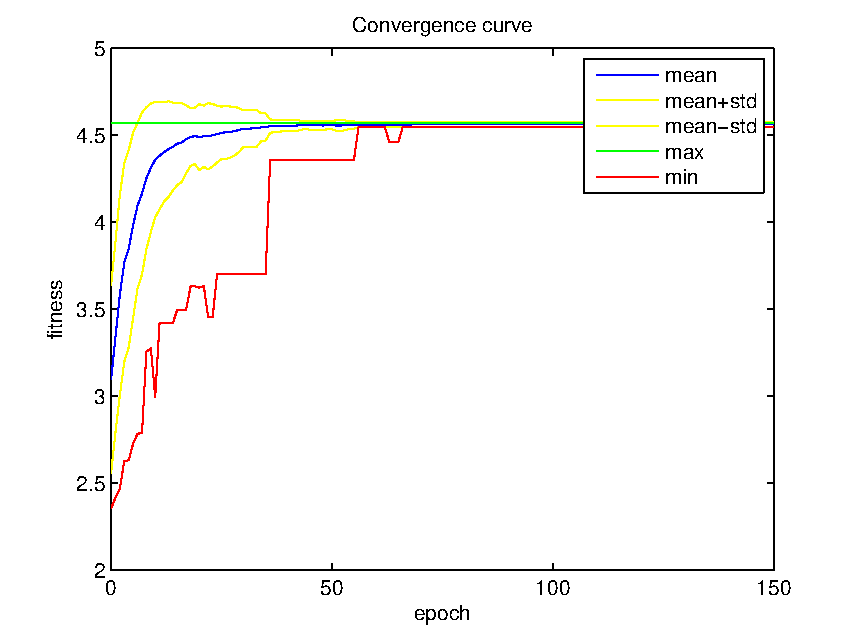
\includegraphics[width=80mm]{ga_conv_curve}
		\label{ga_conv_curve}
	\end{figure}
\end{frame}

\section{Discussion}
\begin{frame}{Discussion}
	\begin{center}
	
		\textbf{Project:}\\\url{https://github.com/pborky/biosiglab}\\
		\textbf{Documents:}\\ \url{https://github.com/pborky/school/tree/master/BIA}\\
		\textbf{Contact:}\\\url{http://www.pborky.sk/contact}\\
	
	\end{center}
\end{frame}

\end{document}